\section{Computer Engineering}

\begin{concept}{What is Computer Engineering?}\\
Computer Engineering is where microelectronics and software meet. It involves:
\begin{itemize}
  \item Architecture and organization of computer systems
  \item Combines hardware and software to implement a computer
  \item Applications in embedded systems, information technology, and technical/scientific tools
\end{itemize}
\end{concept}

\begin{definition}{Basic Hardware Components}\\
A computer system consists of four fundamental components:
\begin{itemize}
  \item \textbf{CPU (Central Processing Unit)}: Processes instructions and data
  \item \textbf{Memory}: Stores instructions and data
  \item \textbf{Input/Output}: Interface to external devices
  \item \textbf{System Bus}: Electrical connection between components
\end{itemize}

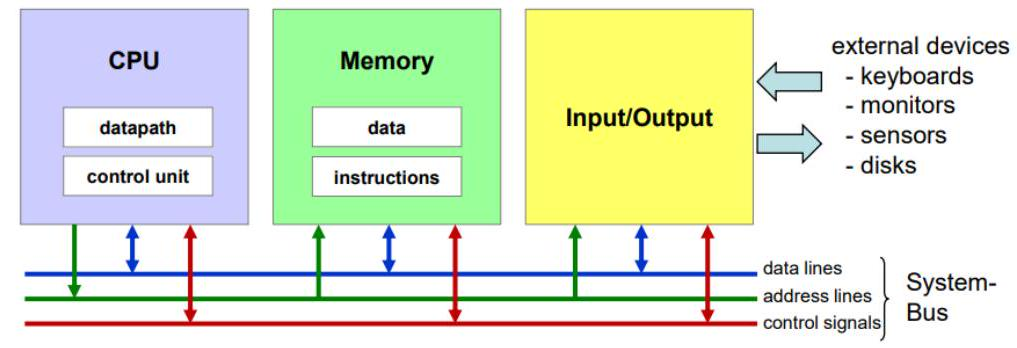
\includegraphics[width=\linewidth]{images/2024_12_29_79e6b22f503fb7b4f718g-01(1)}
\end{definition}

\begin{definition}{CPU Components}\\
The CPU contains several key components:
\begin{itemize}
  \item \textbf{Core Registers}: Fast but limited storage inside CPU
  \item \textbf{ALU (Arithmetic Logic Unit)}: Performs arithmetic and logic operations
  \item \textbf{Control Unit}: Reads and executes instructions
  \item \textbf{Bus Interface}: Connects CPU to system bus
\end{itemize}
\end{definition}

\begin{concept}{Memory Types}
\begin{itemize}
  \item \textbf{Main Memory (Arbeitsspeicher)}:
    \begin{itemize}
      \item Connected through System-Bus
      \item Access to individual bytes
      \item Volatile: SRAM, DRAM
      \item Non-volatile: ROM, Flash
    \end{itemize}
  \item \textbf{Secondary Storage}:
    \begin{itemize}
      \item Connected through I/O
      \item Access to blocks of data
      \item Non-volatile
      \item Examples: HDD, SSD, CD, DVD
    \end{itemize}
\end{itemize}
\end{concept}

\begin{formula}{Program Translation Process}\\
Translation from source code to executable involves four steps:

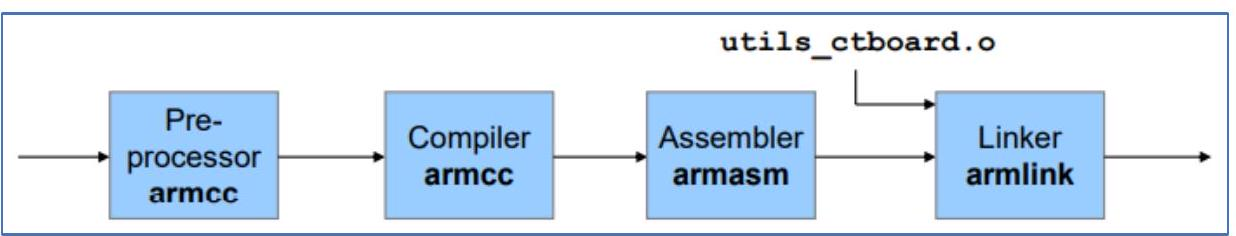
\includegraphics[width=\linewidth]{images/2024_12_29_79e6b22f503fb7b4f718g-01}

\begin{enumerate}
  \item \textbf{Preprocessor}:
    \begin{itemize}
      \item Text processing
      \item Includes header files
      \item Expands macros
      \item Output: Modified source program
    \end{itemize}
  \item \textbf{Compiler}:
    \begin{itemize}
      \item Translates C to assembly
      \item CPU-specific code generation
      \item Output: Assembly program
    \end{itemize}
  \item \textbf{Assembler}:
    \begin{itemize}
      \item Converts assembly to machine code
      \item Creates relocatable object file
      \item Output: Binary object file
    \end{itemize}
  \item \textbf{Linker}:
    \begin{itemize}
      \item Merges object files
      \item Resolves dependencies
      \item Creates executable program
      \item Output: Executable file
    \end{itemize}
\end{enumerate}
\end{formula}

\begin{KR}{Program Compilation Process}\\
To compile and link a program:
\begin{enumerate}
  \item Create source files (.c) and header files (.h)
  \item Run preprocessor to expand includes and macros
  \item Compile source files to object files
  \item Link object files and libraries
  \item Test executable
\end{enumerate}
\end{KR}

\begin{code}{Simple Program Translation - From Source to Executable}
\begin{lstlisting}[language=C, style=base]
#include <stdio.h>
#define MAX 100

int main(void) {
    printf("Max is %d\n", MAX);
    return 0;
}
\end{lstlisting}

Translation steps:
\begin{enumerate}
  \item Preprocessor expands include and replaces MAX with 100
  \item Compiler converts to assembly language
  \item Assembler creates object file
  \item Linker combines with C library to create executable
\end{enumerate}
\end{code}